\let\negmedspace\undefined
\let\negthickspace\undefined
\documentclass[journal,12pt,twocolumn]{IEEEtran}
\usepackage{gensymb}
\usepackage{amssymb}
\usepackage[cmex10]{amsmath}
\usepackage{amsthm}
\usepackage[export]{adjustbox}
\usepackage{bm}
\usepackage{longtable}
\usepackage{enumitem}
\usepackage{mathtools}
 \usepackage{tikz}
\usepackage[breaklinks=true]{hyperref}
\usepackage{listings}
\usepackage{color}                                            %%
\usepackage{array}                                            %%
\usepackage{longtable}                                        %%
\usepackage{calc}                                             %%
\usepackage{multirow}                                         %%
\usepackage{hhline}                                           %%
\usepackage{ifthen}                                           %%
\usepackage{lscape}     
\usepackage{multicol}
% \usepackage{enumerate}
\DeclareMathOperator*{\Res}{Res}
\renewcommand\thesection{\arabic{section}}
\renewcommand\thesubsection{\thesection.\arabic{subsection}}
\renewcommand\thesubsubsection{\thesubsection.\arabic{subsubsection}}
\renewcommand\thesectiondis{\arabic{section}}
\renewcommand\thesubsectiondis{\thesectiondis.\arabic{subsection}}
\renewcommand\thesubsubsectiondis{\thesubsectiondis.\arabic{subsubsection}}
\hyphenation{op-tical net-works semi-conduc-tor}
\def\inputGnumericTable{}                                 %%
\lstset{
frame=single, 
breaklines=true,
columns=fullflexible
}
\newtheorem{theorem}{Theorem}[section]
\newtheorem{problem}{Problem}
\newtheorem{proposition}{Proposition}[section]
\newtheorem{lemma}{Lemma}[section]
\newtheorem{corollary}[theorem]{Corollary}
\newtheorem{example}{Example}[section]
\newtheorem{definition}[problem]{Definition}
\newcommand{\BEQA}{\begin{eqnarray}}
\newcommand{\EEQA}{\end{eqnarray}}
\newcommand{\define}{\stackrel{\triangle}{=}}
\newcommand*\circled[1]{\tikz[baseline=(char.base)]{
    \node[shape=circle,draw,inner sep=2pt] (char) {#1};}}
\bibliographystyle{IEEEtran}
\providecommand{\mbf}{\mathbf}
\providecommand{\pr}[1]{\ensuremath{\Pr\left(#1\right)}}
\providecommand{\qfunc}[1]{\ensuremath{Q\left(#1\right)}}
\providecommand{\sbrak}[1]{\ensuremath{{}\left[#1\right]}}
\providecommand{\lsbrak}[1]{\ensuremath{{}\left[#1\right.}}
\providecommand{\rsbrak}[1]{\ensuremath{{}\left.#1\right]}}
\providecommand{\brak}[1]{\ensuremath{\left(#1\right)}}
\providecommand{\lbrak}[1]{\ensuremath{\left(#1\right.}}
\providecommand{\rbrak}[1]{\ensuremath{\left.#1\right)}}
\providecommand{\cbrak}[1]{\ensuremath{\left\{#1\right\}}}
\providecommand{\lcbrak}[1]{\ensuremath{\left\{#1\right.}}
\providecommand{\rcbrak}[1]{\ensuremath{\left.#1\right\}}}
\theoremstyle{remark}
\newtheorem{rem}{Remark}
\newcommand{\sgn}{\mathop{\mathrm{sgn}}}
\providecommand{\abs}[1]{\left\vert#1\right\vert}
\providecommand{\res}[1]{\Res\displaylimits_{#1}} 
\providecommand{\norm}[1]{\left\lVert#1\right\rVert}
%\providecommand{\norm}[1]{\lVert#1\rVert}
\providecommand{\mtx}[1]{\mathbf{#1}}
\providecommand{\mean}[1]{E\left[ #1 \right]}
\providecommand{\fourier}{\overset{\mathcal{F}}{ \rightleftharpoons}}
%\providecommand{\hilbert}{\overset{\mathcal{H}}{ \rightleftharpoons}}
\providecommand{\system}{\overset{\mathcal{H}}{ \longleftrightarrow}}
	%\newcommand{\solution}[2]{\textbf{Solution:}{#1}}
\newcommand{\solution}{\noindent \textbf{Solution: }}
\newcommand{\cosec}{\,\text{cosec}\,}
\providecommand{\dec}[2]{\ensuremath{\overset{#1}{\underset{#2}{\gtrless}}}}
\newcommand{\myvec}[1]{\ensuremath{\begin{pmatrix}#1\end{pmatrix}}}
\newcommand{\mydet}[1]{\ensuremath{\begin{vmatrix}#1\end{vmatrix}}}
\newcommand*{\permcomb}[4][0mu]{{{}^{#3}\mkern#1#2_{#4}}}
\newcommand*{\perm}[1][-3mu]{\permcomb[#1]{P}}
\newcommand*{\comb}[1][-1mu]{\permcomb[#1]{C}}
\numberwithin{equation}{subsection}
\makeatletter
\@addtoreset{figure}{problem}
\makeatother
\let\StandardTheFigure\thefigure
\let\vec\mathbf
\renewcommand{\thefigure}{\theproblem}
\def\putbox#1#2#3{\makebox[0in][l]{\makebox[#1][l]{}\raisebox{\baselineskip}[0in][0in]{\raisebox{#2}[0in][0in]{#3}}}}
     \def\rightbox#1{\makebox[0in][r]{#1}}
     \def\centbox#1{\makebox[0in]{#1}}
     \def\topbox#1{\raisebox{-\baselineskip}[0in][0in]{#1}}
     \def\midbox#1{\raisebox{-0.5\baselineskip}[0in][0in]{#1}}
\vspace{3cm}

\title{AI1110 ASSIGNMENT 1}
\author{Bandaru Naresh Kumar, AI21BTECH11006}
\begin{document}
\maketitle
\textbf{ICSE class 10 paper 2019}\\\\
\textbf{Q3 (b):}
$\vec{M}$ and $\vec{N}$ are two points on the X axis and Y axis respectively.
$\vec{P}(3,2)$ divides the line segment MN in the ratio 2:3.\\
Find:\\
 (i)the coordinates of $\vec{M}$ and $\vec{N}$\\
 (ii)the slope of MN.\\\\
\\\textbf{Solution:}\\
\begin{table}[ht]
\centering
\begin{tabular}{|c|c|c|}
\hline
Symbol & Value & Description\\
\hline
\hline
P & $\myvec{3\\2}$ & Given point\\
\hline
$e_1$ & $\myvec{1\\0}$ & Standard X-axis vector\\
\hline
$e_2$ & $\myvec{0\\1}$ & Standard Y-axis vector\\
\hline
M & $ae_1$ & A point on X-axis and $a\in R$\\
\hline
N & $be_2$ & A point on Y-axis and $b\in R$\\
\hline
k & $\dfrac{2}{3}$ & Ratio in which P divides MN\\
\hline
\end{tabular}
\caption{variables}
\label{tab:variables}
\end{table}
Various paraetres used in this question are:\\
According to Section formula,\\
If $\vec{P}$ divides MN in the ratio k:1,then:
\begin{align}
   \vec{P} &= \dfrac{k(\vec{N})+1(\vec{M})}{k+1}\\
   \vec{P} &= \dfrac{bk\vec{e_2}+a\vec{e_1}}{k+1}\\
   \vec{P} &= \left( \dfrac{a}{k+1}\right) \vec{e_1}+\left( \dfrac{bk}{k+1}\right) \vec{e_2}
\end{align}\\
But we have,\\
 $ \vec{P} = \myvec{3 \\ 2}$\\
\begin{figure}[h]
\centering  
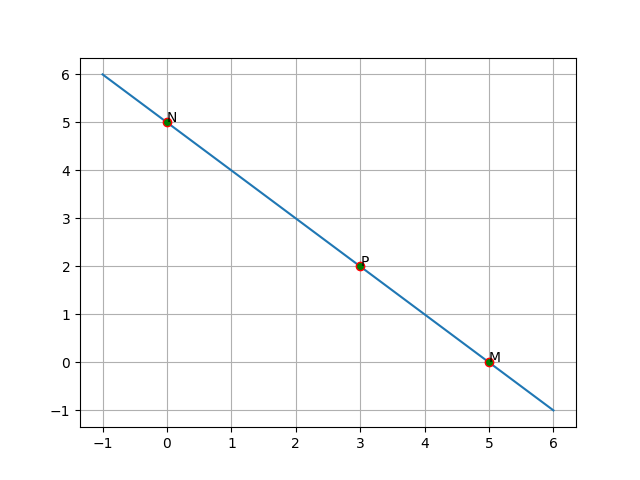
\includegraphics[width=\columnwidth]{figures/Figure_1.png} 
\end{figure}
Therefore,
\begin{align}
 \left( \dfrac{a}{k+1}\right) \vec{e_1}+\left( \dfrac{bk}{k+1}\right) \vec{e_2} &= \myvec{3 \\ 2}\\
 \left( \dfrac{a}{k+1}\right) \vec{e_1}+\left( \dfrac{bk}{k+1}\right) \vec{e_2} &= 3\vec{e_1}+2\vec{e_2}
\end{align}
  $\implies$ $\dfrac{a}{k+1} = 3$ and $\dfrac{bk}{k+1} = 2$\\\\
  $\implies$ $a = 3(k+1)$ and $b = \dfrac{2(k+1)}{k}$\\\\ 
Substituting $k = \dfrac{2}{3}$ , we get:\\
   $a = 5$ and $b = 5$\\\\
(i)$\vec{M} = 5\vec{e_1}$ and $\vec{N} = 5\vec{e_2}$\\\\
(ii) Slope of MN = $\dfrac{5-0}{0-5}$\\\\
     \hspace*{85pt} = -1
\end{document}